% =====================================================================
% Boutique Pipeline — Hebrew User Guide (image-first rewrite, standalone).
% Compile with XeLaTeX:
%   xelatex boutique_pipeline_guide_hebrew.tex
% =====================================================================

\documentclass[11pt,a4paper]{article}

\usepackage{fontspec}
\usepackage{polyglossia}
\setdefaultlanguage{hebrew}
\setotherlanguage{english}

\newfontfamily\hebrewfont[Script=Hebrew]{David}
\newfontfamily\hebrewfontsf[Script=Hebrew]{Arial}
\newfontfamily\hebrewfonttt[Script=Hebrew]{Courier New}
\newfontfamily\englishfont{Times New Roman}

\usepackage{amsmath,amssymb}
\usepackage{graphicx}
\usepackage{float}
\usepackage{booktabs}
\usepackage[table]{xcolor}
\usepackage{array}
\usepackage{hyperref}
\usepackage[margin=2cm]{geometry}

\graphicspath{{figures/}}

\hypersetup{
  colorlinks=true,
  linkcolor=blue!50!black,
  urlcolor=blue!50!black,
  pdftitle={Boutique Pipeline - Hebrew User Guide},
}

\title{\textbf{מדריך שימוש: פייפליין בוטיק}\\
{\large הערכת מרחק אנכי במעלית מרשומת חיישני סמארטפון}}
\author{אייל יקיר \and אוריה כהן-אליה}
\date{\today}

\begin{document}

\maketitle

\begin{abstract}
\noindent
מדריך מעשי, מבוסס תמונות, ל-\textenglish{Streamlit} של פייפליין בוטיק
(\textenglish{\texttt{src/pipelines/boutique\_pipeline.py}}). המסמך
מציג את האפליקציה צעד אחר צעד עם צילומי מסך אמיתיים, ובכל בדיקת
``האם הסגמנט תקין'' מובאת השוואה זה-לצד-זה של דוגמה טובה לעומת
דוגמה גרועה. אם כל מה שמעניין אותך הוא להפיק דו"ח --- קרא רק את
\autoref{sec:heb-quickstart} ואז את \autoref{sec:heb-good-vs-bad};
כל שאר הסעיפים הם רשות.
\end{abstract}

\tableofcontents
\bigskip

% =====================================================================
\section{התחלה מהירה: חמש לחיצות עד דו"ח}
\label{sec:heb-quickstart}

\paragraph{הפעלה.}
משורש הפרויקט, עם הסביבה הוירטואלית פעילה:

\begin{verbatim}
venv/bin/python -m streamlit run src/pipelines/boutique_pipeline.py
\end{verbatim}

\noindent\textenglish{Streamlit} ידפיס כתובת מקומית
(ברירת מחדל \textenglish{\texttt{http://localhost:8501}}).
האשף מתקדם דרך הכפתור הראשי שבפינה הימנית-תחתונה של כל עמוד
(\textenglish{Next \textrightarrow}, \textenglish{Predict
\textrightarrow}, \textenglish{Generate report \textrightarrow}).

% ---------- Step 1 ----------
\begin{figure}[H]
\centering
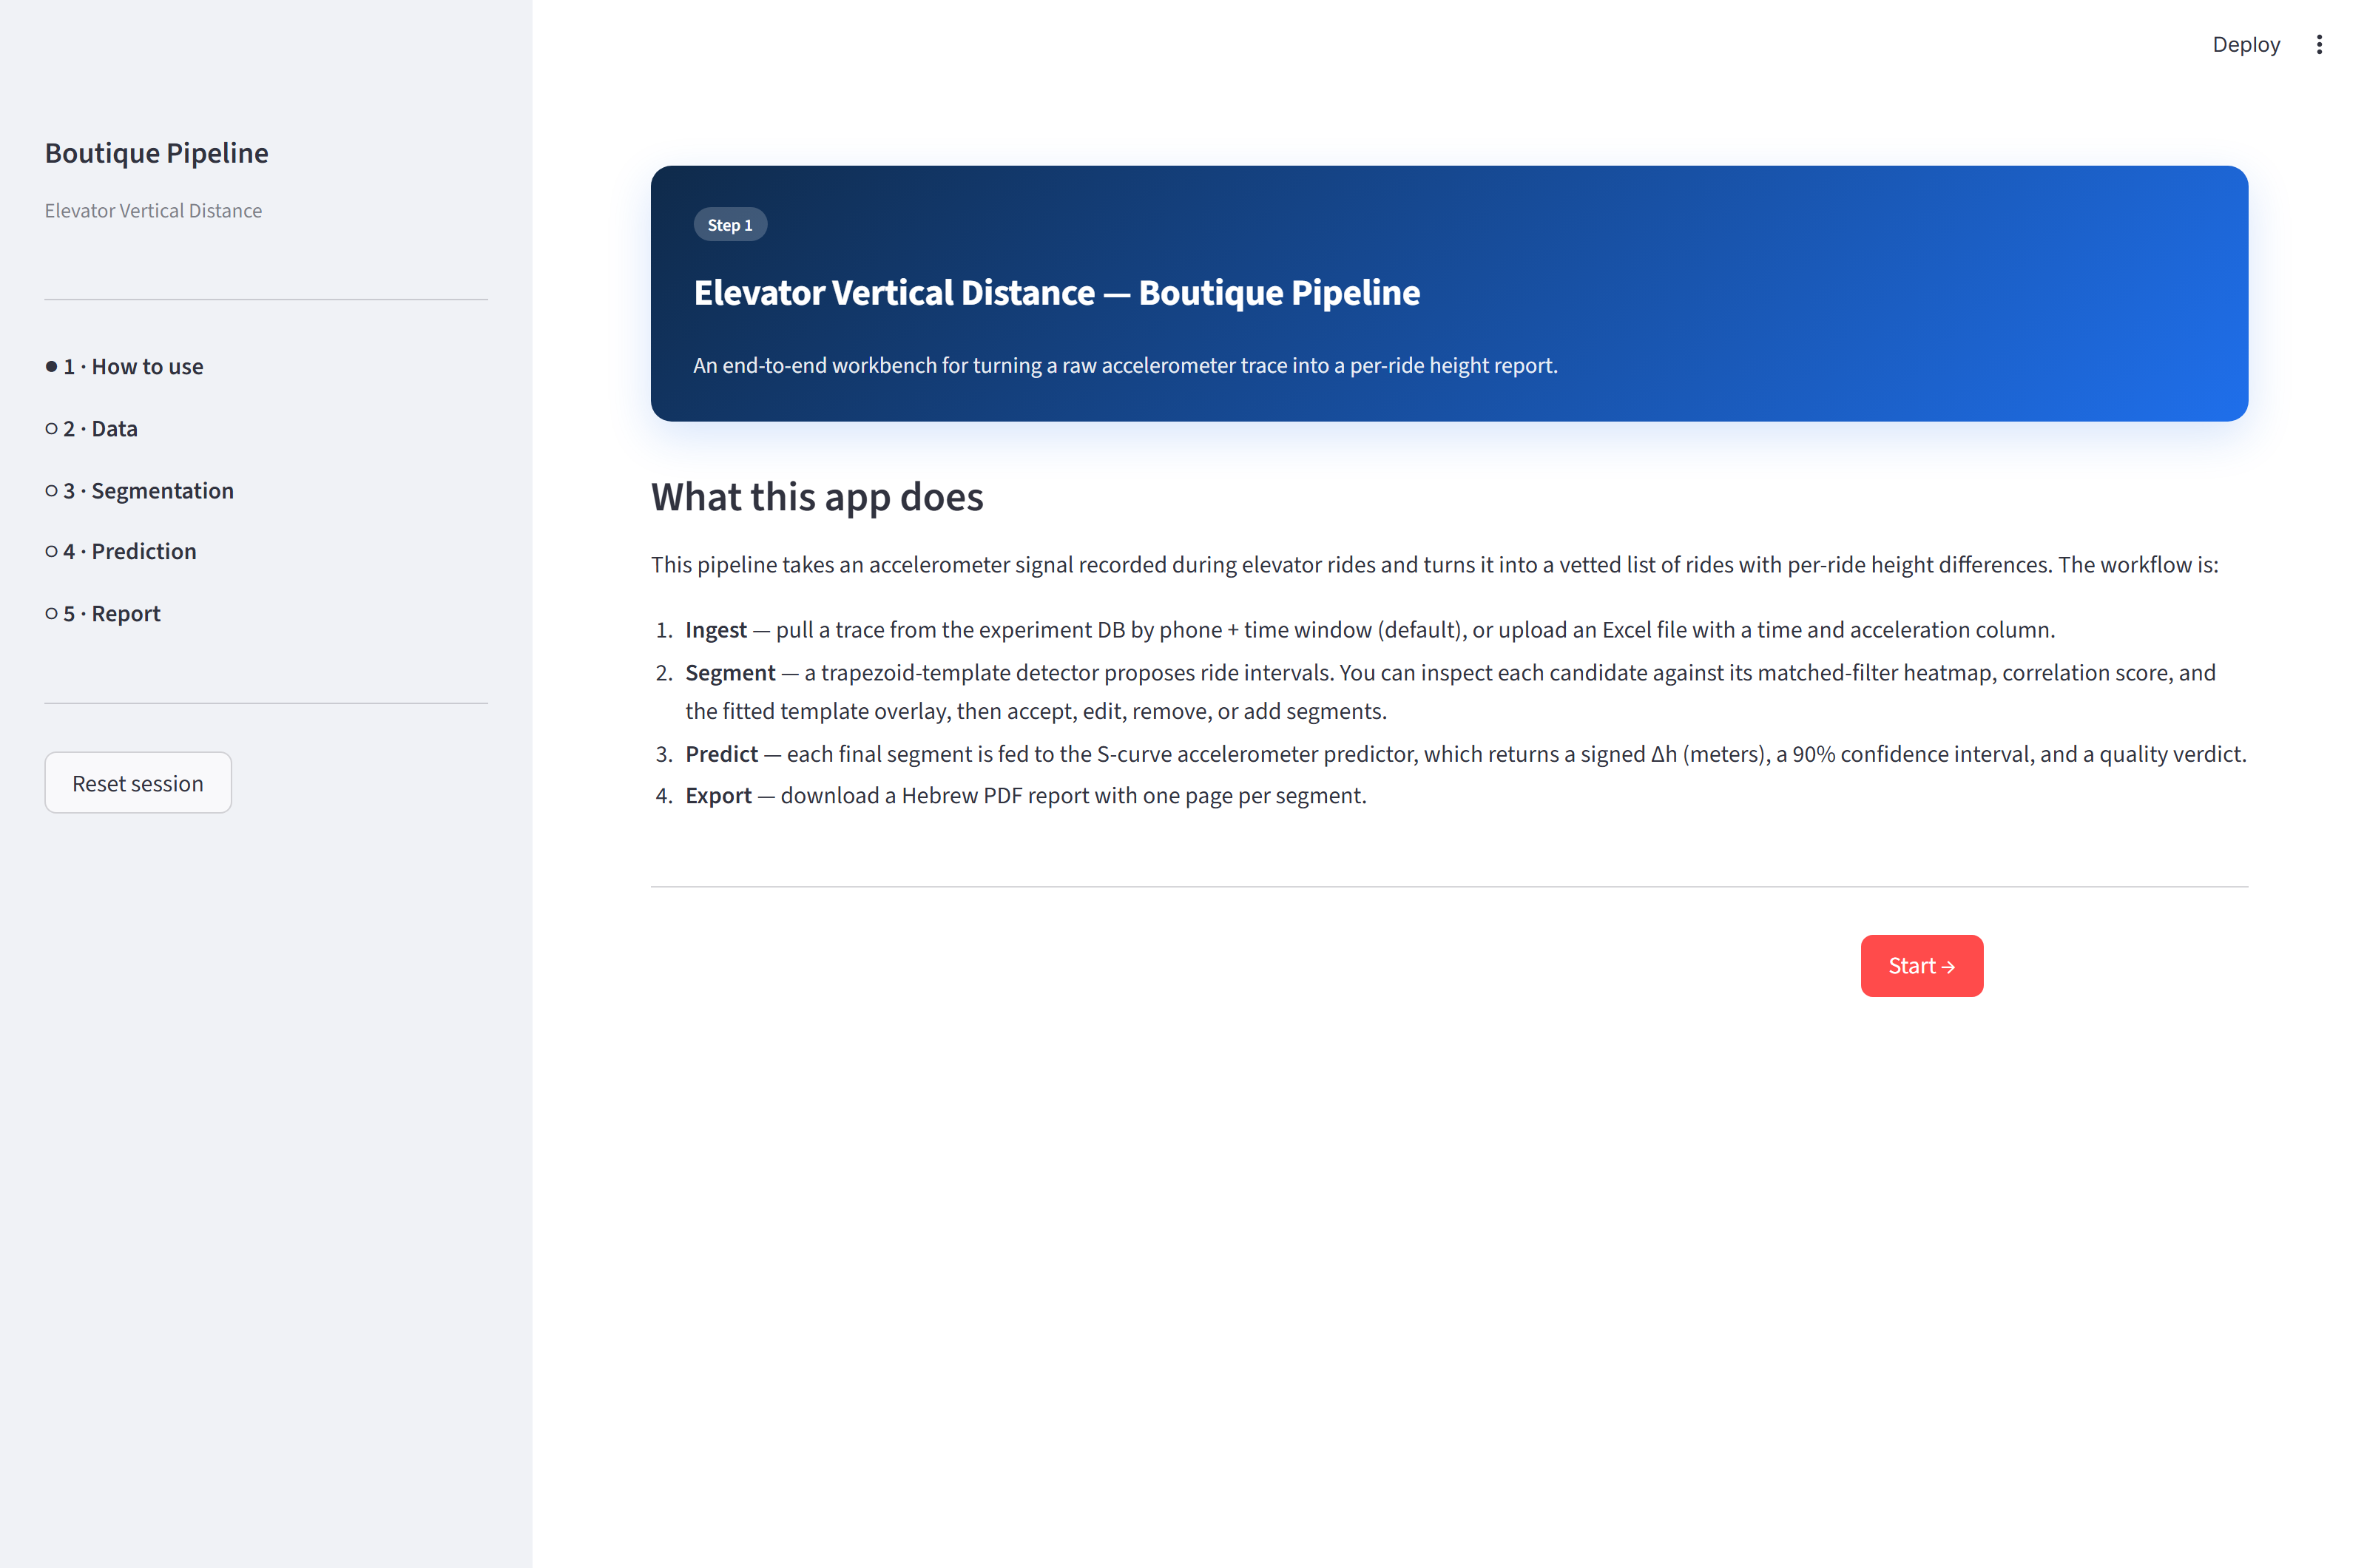
\includegraphics[width=0.95\linewidth]{boutique/ui_step1_landing.png}
\caption{\textbf{שלב 1 --- דף פתיחה.} פסקה אחת של רקע. לוחצים
\textenglish{Start \textrightarrow}.}
\label{fig:hb-step1}
\end{figure}

% ---------- Step 2 ----------
\begin{figure}[H]
\centering
\begin{minipage}[t]{0.49\linewidth}
\centering
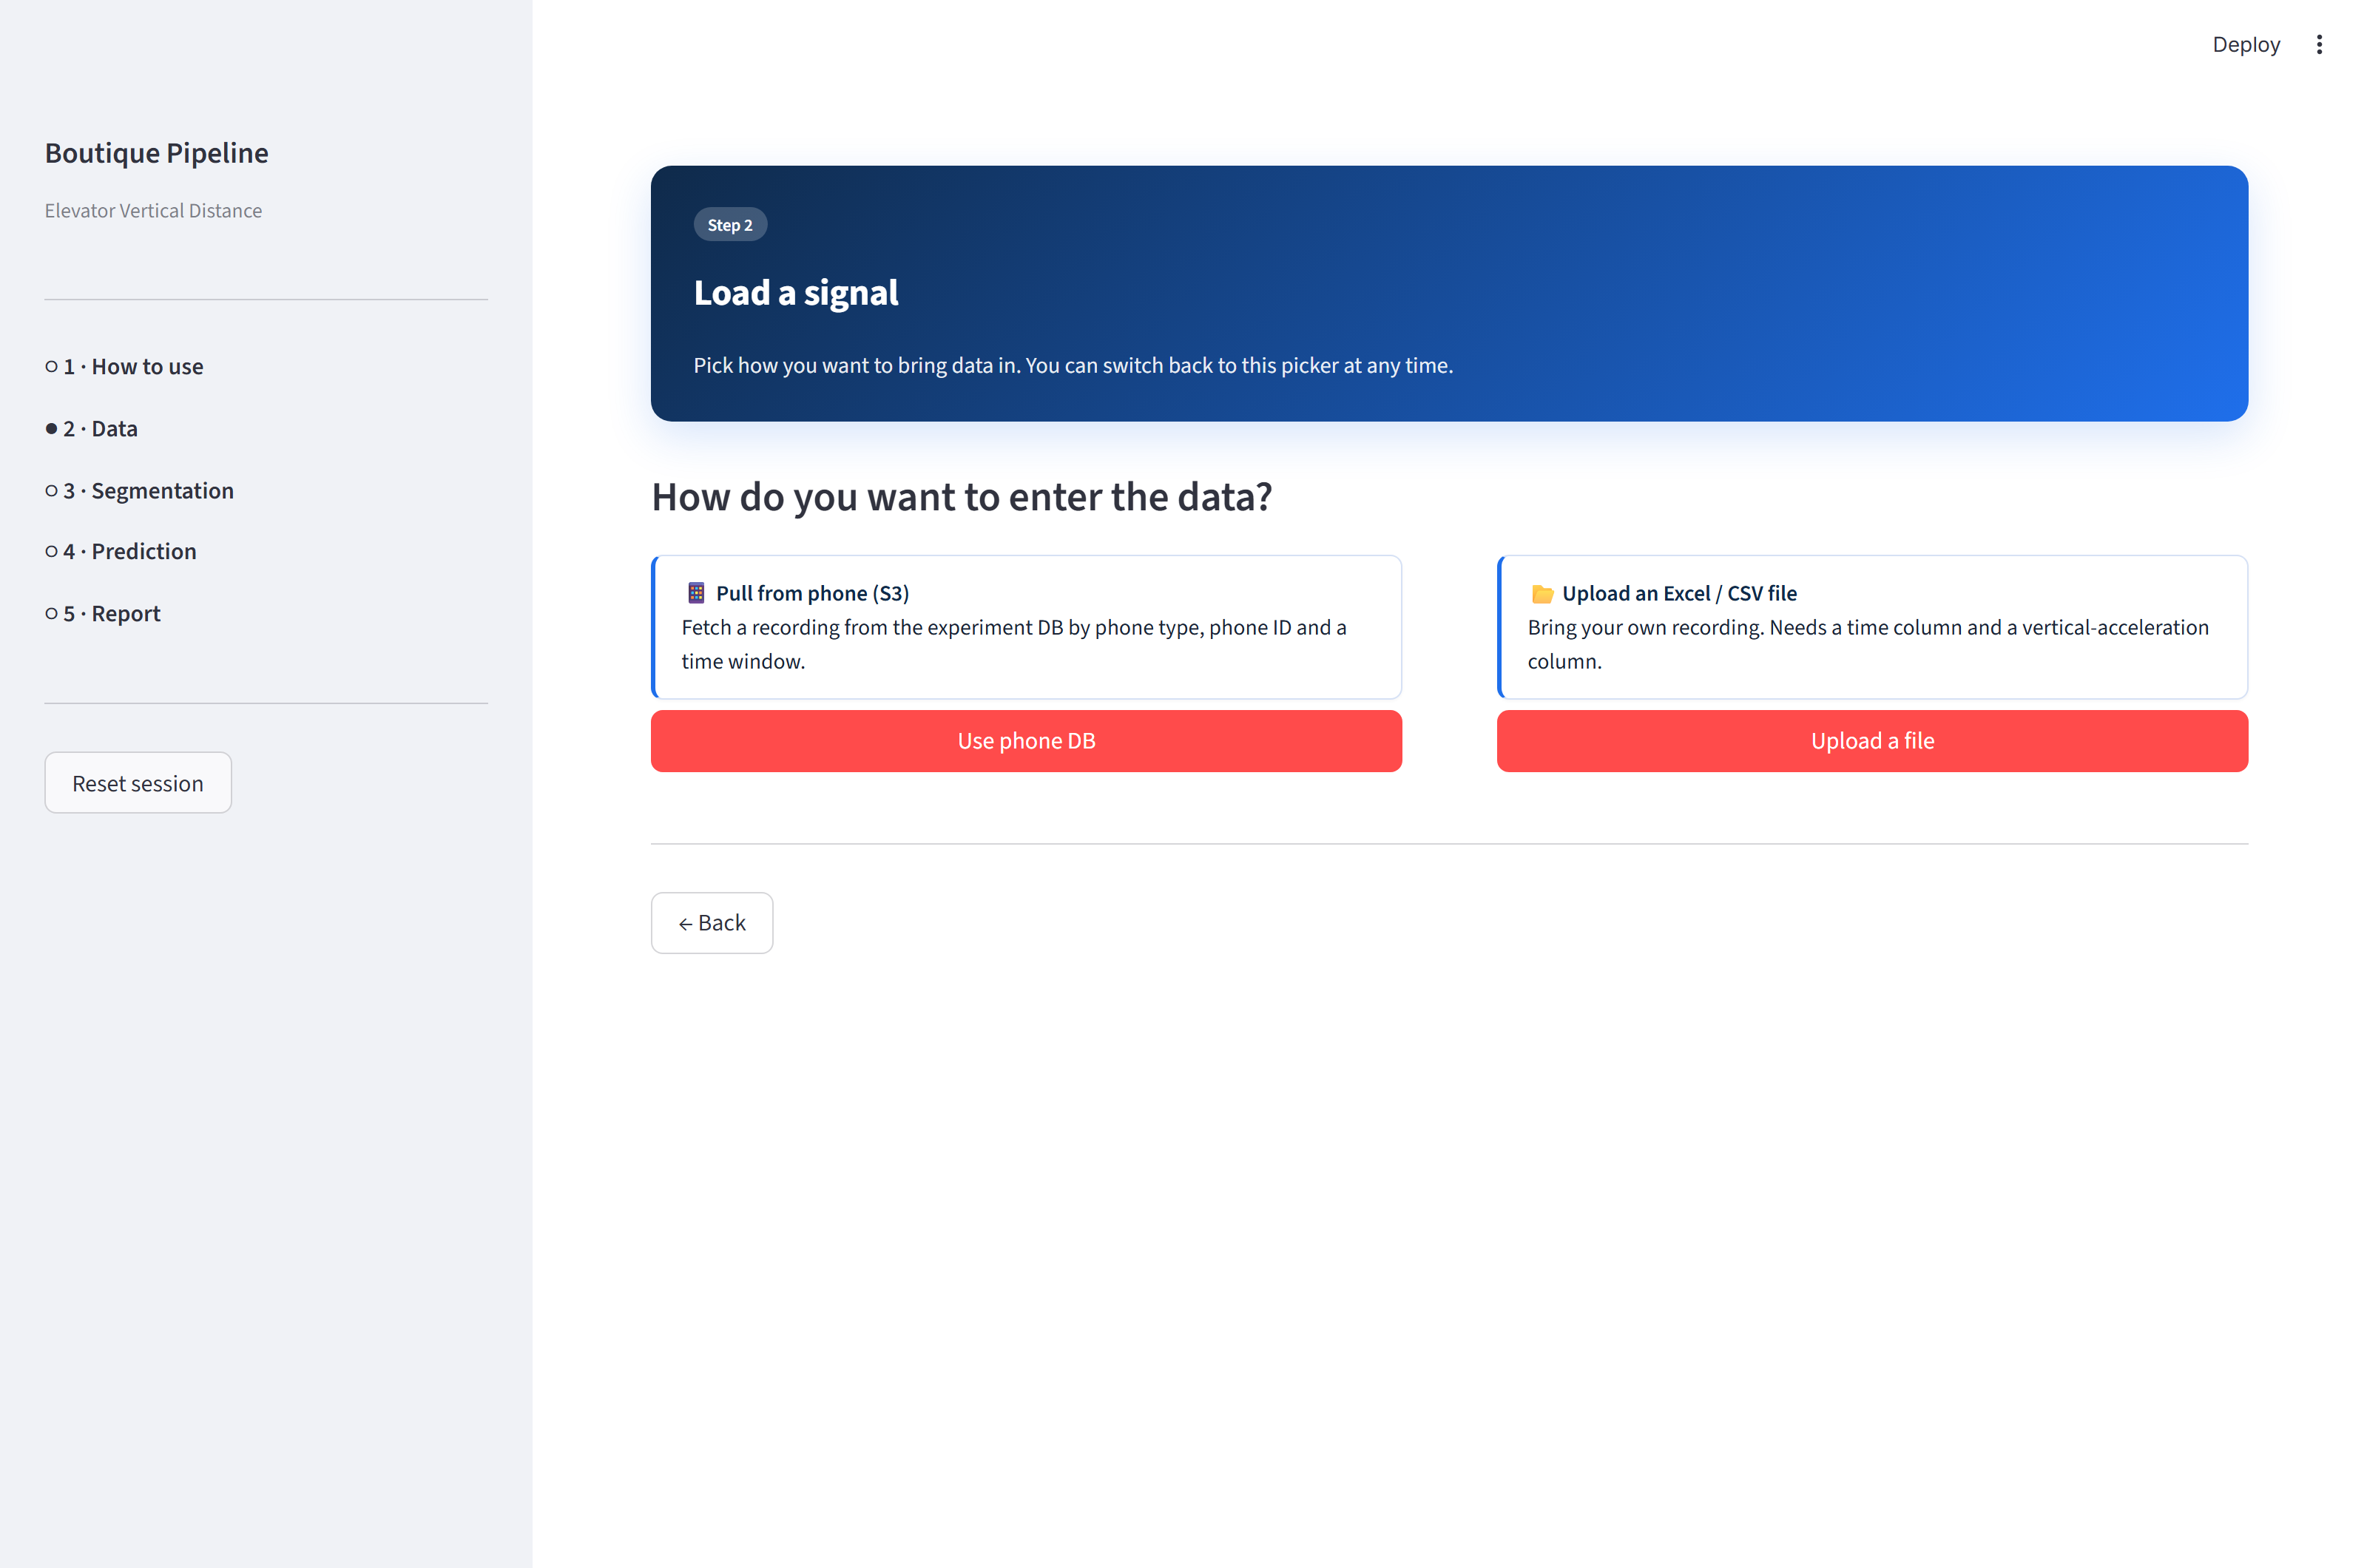
\includegraphics[width=\linewidth]{boutique/ui_step2_picker.png}
\par\smallskip
\textbf{2א.} בוחרים: \textenglish{Use phone DB} (משתמשים פנימיים)
או \textenglish{Upload a file} (כל השאר).
\end{minipage}
\hfill
\begin{minipage}[t]{0.49\linewidth}
\centering
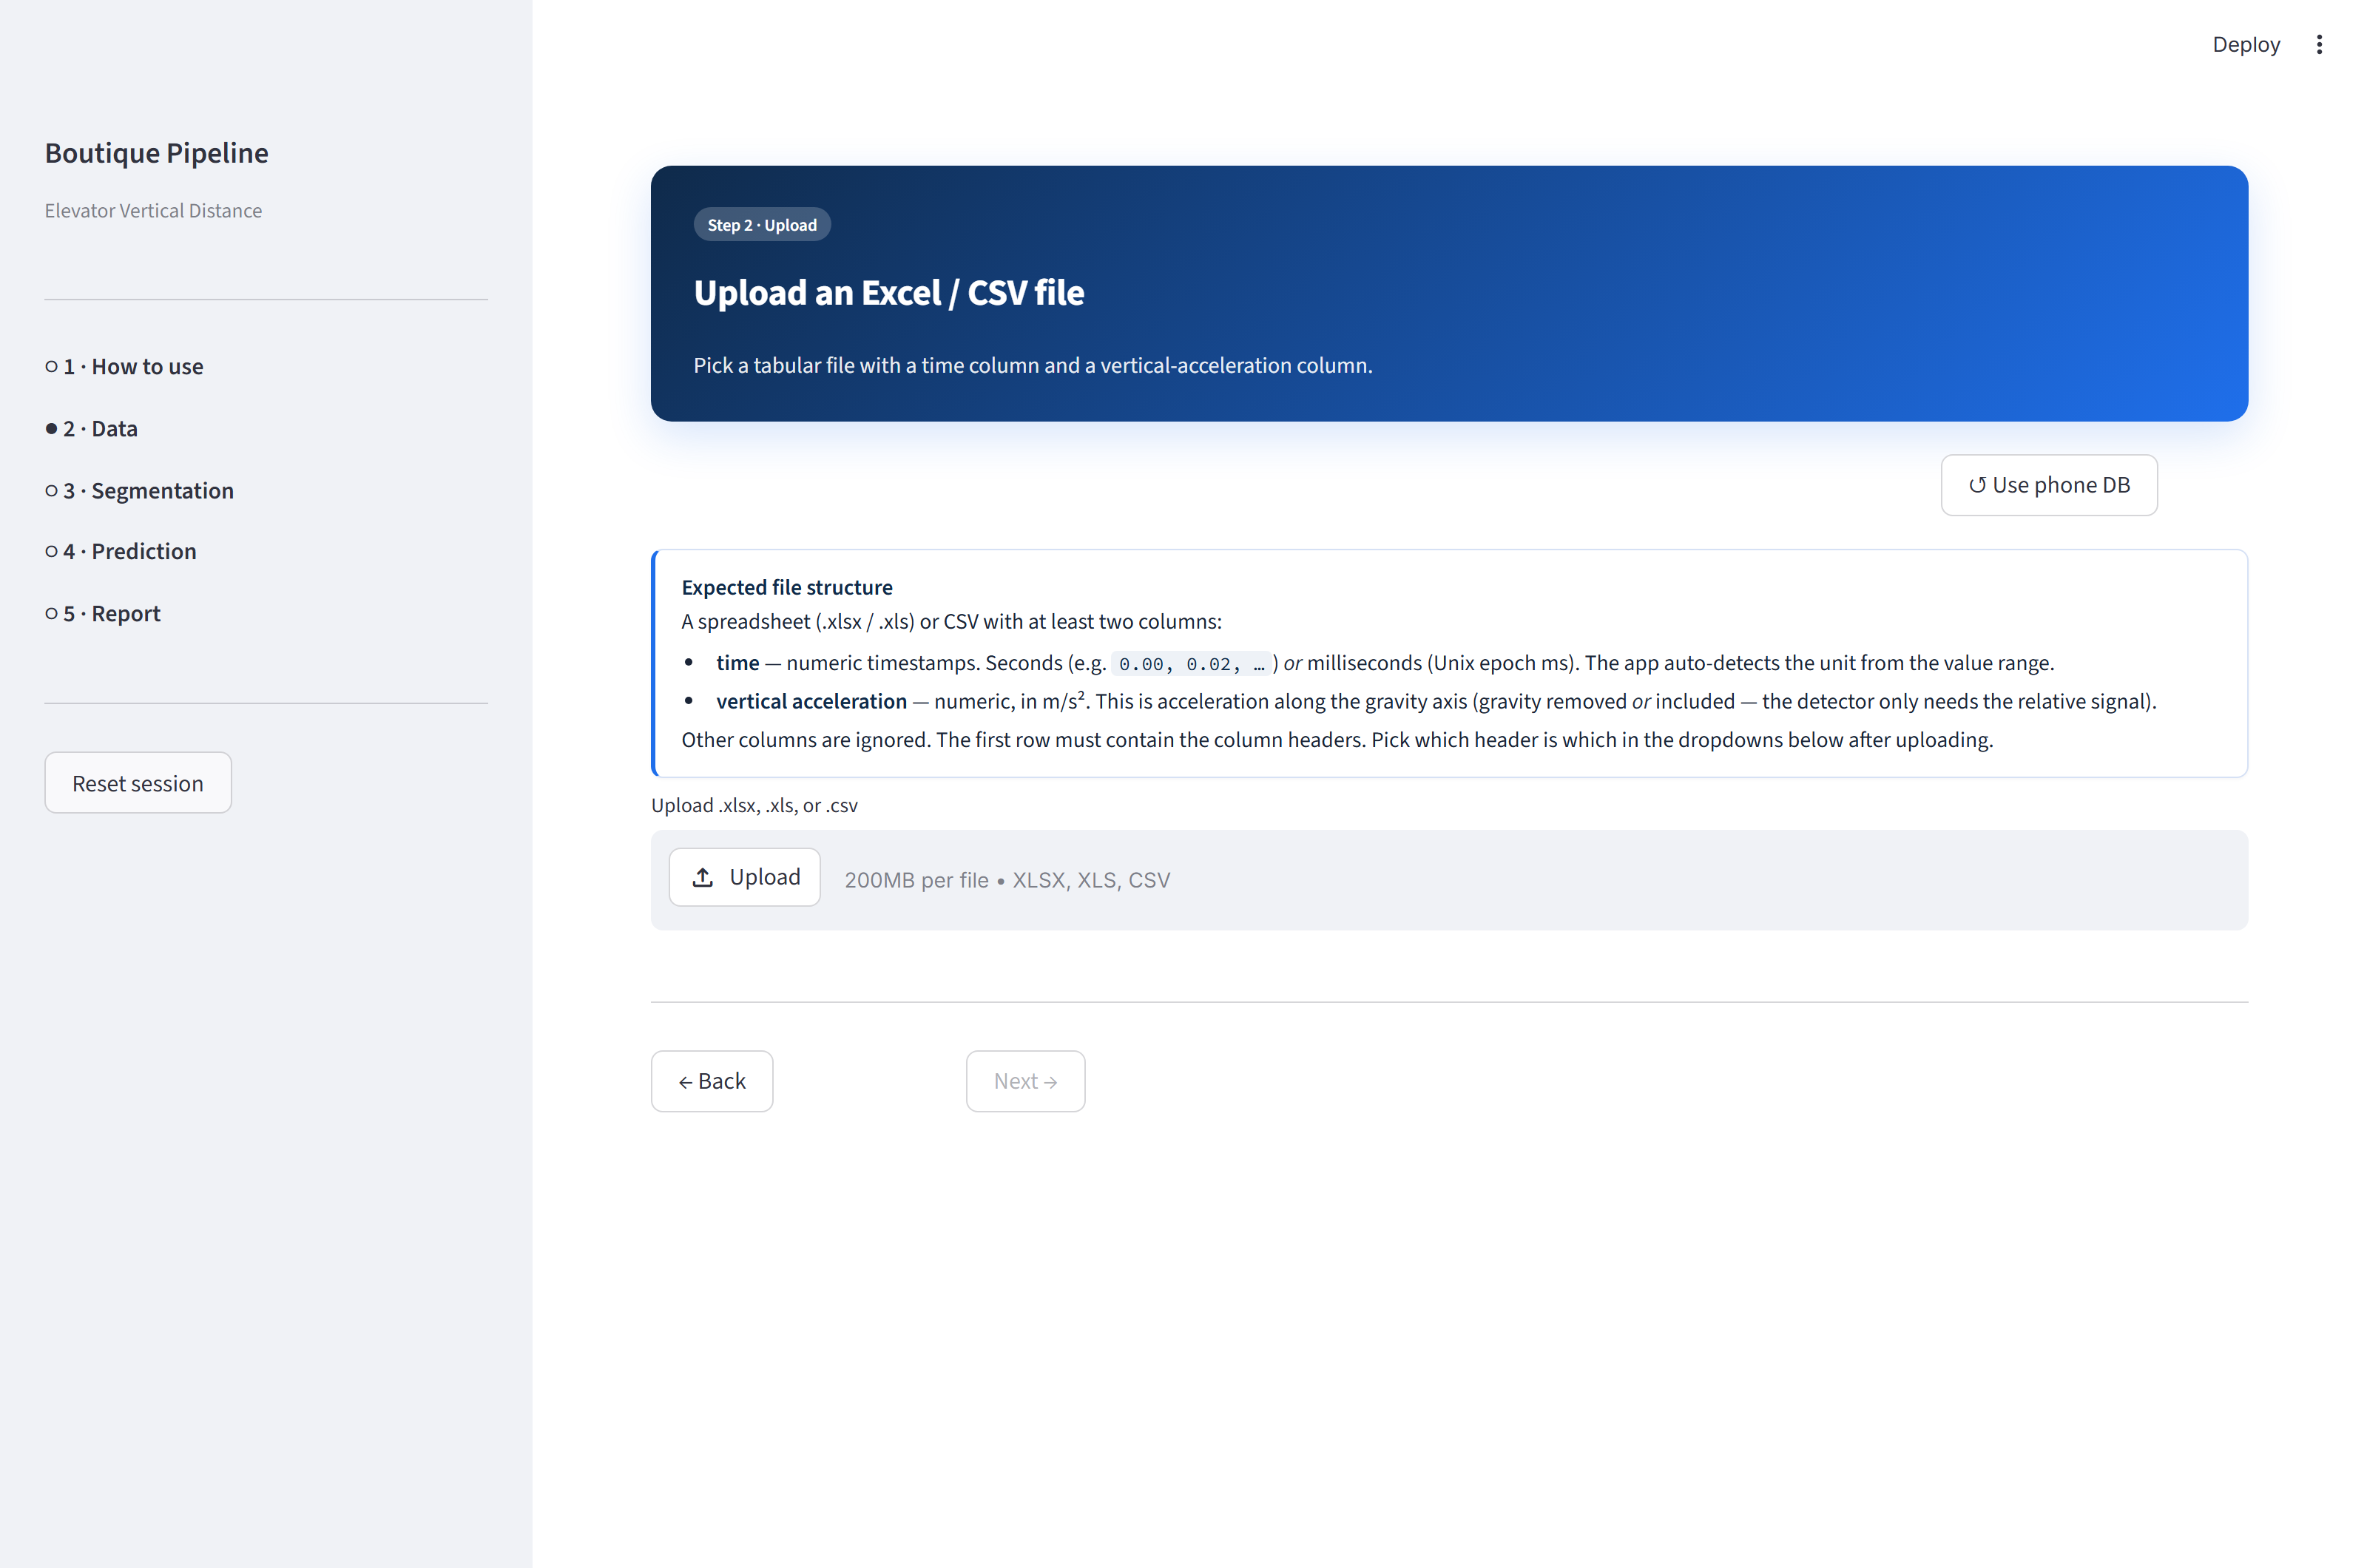
\includegraphics[width=\linewidth]{boutique/ui_step2_upload_form.png}
\par\smallskip
\textbf{2ב.} להעלאת קובץ: \textenglish{CSV/XLSX} עם עמודת זמן
(שניות או מילישניות, מזוהה אוטומטית) ועמודת תאוצה אנכית
(\textenglish{m/s$^2$}). שורה ראשונה חייבת להיות
כותרת.
\end{minipage}
\caption{\textbf{שלב 2 --- נתונים.} שני מצבי קלט. ניתן לחזור ולהחליף
ביניהם בכל עת מקישור \textenglish{change input source} בפינה
הימנית-עליונה.}
\label{fig:hb-step2}
\end{figure}

% ---------- Step 3 ----------
\begin{figure}[H]
\centering

\includegraphics[width=0.97\linewidth]{boutique/panels/clean_step3_overview__signal.png}
\caption{\textbf{שלב 3 --- סגמנטציה.} הגלאי רץ אוטומטית. כל נסיעה
שזוהתה מסומנת ברצועה צבעונית
(\textcolor{blue!70!black}{כחול $=$ עליה},
\textcolor{purple!60!red}{ורוד $=$ ירידה}); הסגמנט הנבחר --- בכתום.
אם המקטעים נראים בסדר, לוחצים \textenglish{Predict \textrightarrow}.
אחרת, ראו \autoref{sec:heb-good-vs-bad} ואת
\autoref{sec:heb-fixing}.}
\label{fig:hb-step3}
\end{figure}

% ---------- Step 4 ----------
\begin{figure}[H]
\centering
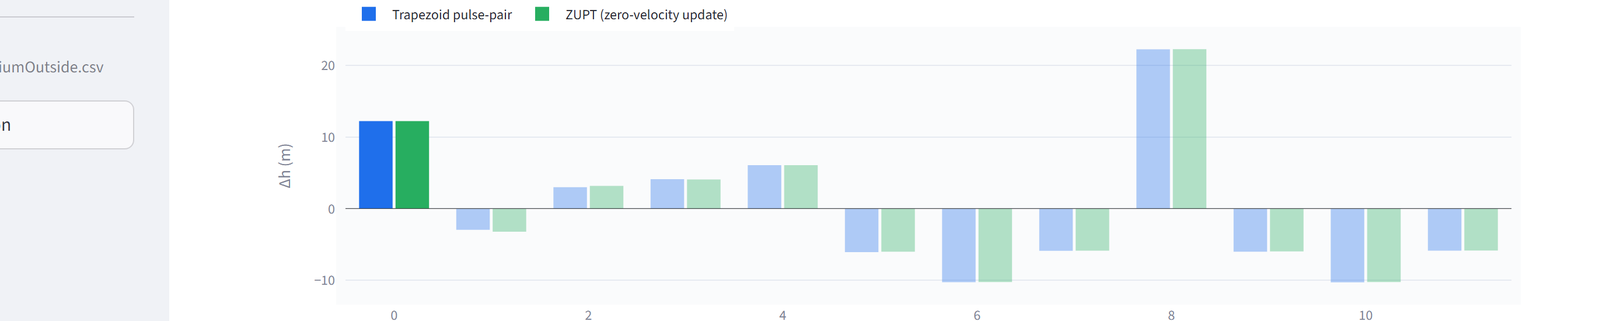
\includegraphics[width=0.95\linewidth]{boutique/crops/clean_step4_metrics.png}
\caption{\textbf{שלב 4 --- חיזוי.} שני האלגוריתמים
(\textenglish{Trapezoid pulse-pair} בכחול, \textenglish{ZUPT}
בירוק) רצים אוטומטית; עמודה אחת לכל אלגוריתם לכל מקטע. עמודה
חיובית $\Rightarrow$ נסיעה כלפי מעלה. שני העמודים אמורים להיות
דומים בגובה. לחיצה על \textenglish{Generate report
\textrightarrow}.}
\label{fig:hb-step4}
\end{figure}

% ---------- Step 5 ----------
\begin{figure}[H]
\centering
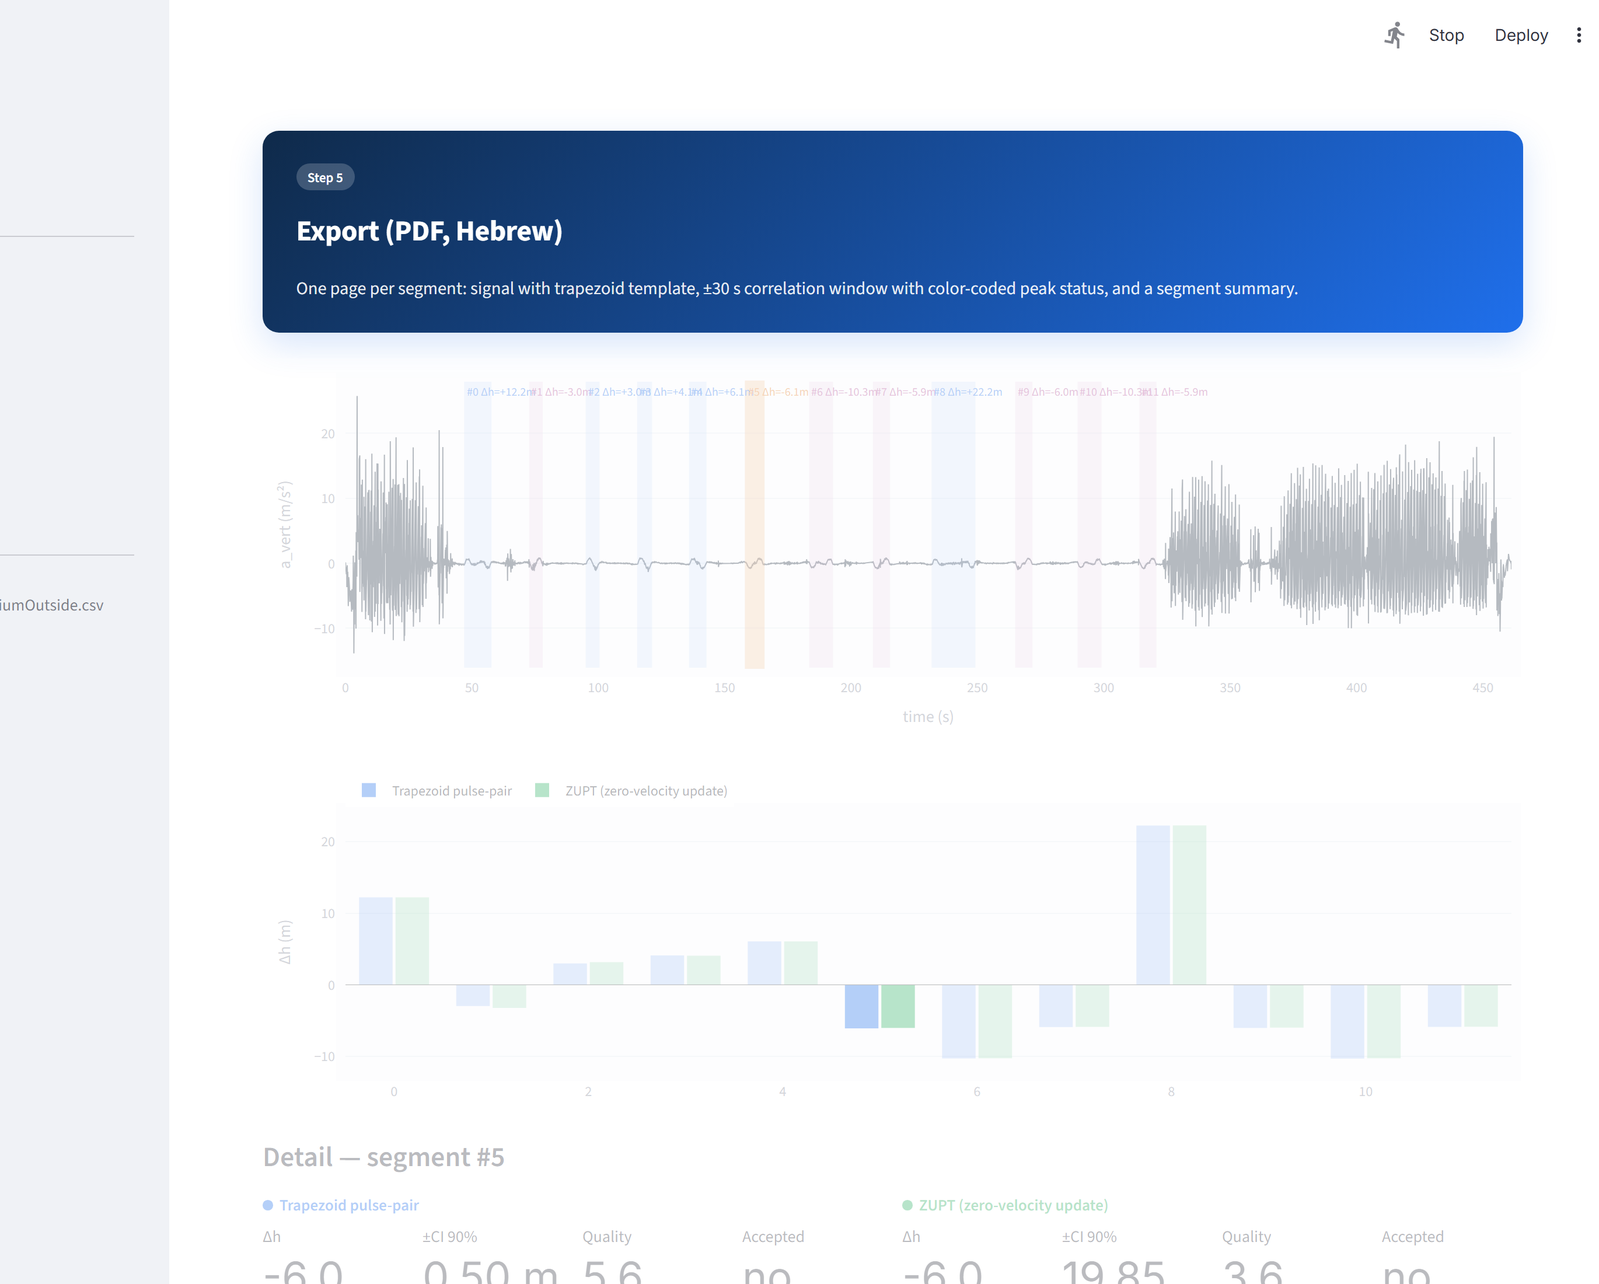
\includegraphics[width=0.85\linewidth]{boutique/crops/clean_step5_top.png}
\caption{\textbf{שלב 5 --- דו"ח.} תצוגה מקדימה של ה-\textenglish{PDF}
מוטמעת בעמוד. לחיצה על \textenglish{Download Summary PDF} שומרת
את הקובץ העברי הסופי.}
\label{fig:hb-step5}
\end{figure}

\paragraph{משפט אחד לכל שלב.}
\begin{enumerate}
  \item קוראים את הרקע הקצר, לוחצים \textenglish{Start}.
  \item בוחרים מקור, לוחצים \textenglish{Next}.
  \item מציצים על המקטעים (הסעיף הבא); אם תקינים ---
    \textenglish{Predict}.
  \item מציצים על תרשים העמודות; אם שני האלגוריתמים מסכימים ---
    \textenglish{Generate report}.
  \item \textenglish{Download}. סיימנו.
\end{enumerate}

\emph{השלב היחיד שמצריך שיקול דעת הוא שלב 3.} הסעיף הבא הוא
``דף הבדיקה'' החזותי שלו.

% =====================================================================
\section{דף בדיקה לשלב 3: האם הסגמנט תקין?}
\label{sec:heb-good-vs-bad}

עמוד הסגמנטציה מציג ארבע חלוניות אבחון מסודרות זו מתחת לזו. בחירת
מקטע (לחיצה על שורה בסרגל הצד או על רצועה צבעונית בגרף העליון)
מרעננת את שלוש החלוניות התחתונות. כל חלונית עונה על שאלת ``כן/לא''
אחת. ביחד --- שניות בודדות לכל החלטה.

% ---- Panel A ----
\subsection{חלונית א --- אות $+$ סגמנטים: האם הנסיעות מכוסות?}

מבט-על על כל ההקלטה. כל נסיעה שזוהתה היא רצועה צבועה; הכתומה היא
הנבחרת.

\begin{figure}[H]
\centering
\begin{minipage}[t]{0.49\linewidth}
\centering

\includegraphics[width=\linewidth]{boutique/panels/clean_step3_overview__signal.png}
\end{minipage}\hfill
\begin{minipage}[t]{0.49\linewidth}
\centering

\includegraphics[width=\linewidth]{boutique/panels/fp_step3_overview__signal.png}
\end{minipage}
\caption{\textbf{אות $+$ סגמנטים.} \emph{שמאל
(\textcolor{green!50!black}{טוב}):} 12 נסיעות נקיות (הקלטת
\textenglish{S23}). כל רצועה יושבת על צורת שתי-אונות ברורה; בין
הרצועות --- אות שקט. אין מה לתקן.
\emph{ימין (\textcolor{red!70!black}{גרוע --- חלוקה עודפת}):}
מקטעים צרים רבים; מקטע 0 הוא קוץ בודד גבוה (תקיעה של הטלפון),
לא נסיעה. המקטעים המאוחרים מצפים תזוזות ידיים רועשות. רובם
צריכים להימחק (\autoref{sec:heb-fixing}, דפוס ב׳).}
\label{fig:hb-overview-cleanvsfp}
\end{figure}

\begin{figure}[H]
\centering

\includegraphics[width=0.97\linewidth]{boutique/panels/damped_step3_overview__signal.png}
\caption{\textbf{\textcolor{red!70!black}{גרוע --- הקלטה
מוחלשת.}} תרחיש ``טלפון בכיס''. הגלאי מצא 10 מקטעים אבל בהקלטה
יש בפועל הרבה יותר נסיעות --- כל קוץ שחור גדול שלא עוטף ברצועה
הוא נסיעה שפוספסה כי המשרעת היתה מתחת לסף. מוסיפים סגמנטים
ידנית (\autoref{sec:heb-fixing}, דפוס א׳).}
\label{fig:hb-overview-damped}
\end{figure}

% ---- Panel B ----
\subsection{חלונית ב --- הטרפז המותאם: האם התבנית מתאימה לאות?}

החלונית התחתונה מתמקדת במקטע הנבחר ומצליבה את שתי תבניות הטרפז
שהותאמו (אונה 1 באדום, אונה 2 בסגול) על האות הגולמי. \emph{זוהי
החלונית האינפורמטיבית ביותר להחלטה האם המקטע אמין.}

\begin{figure}[H]
\centering

\includegraphics[width=0.97\linewidth]{boutique/panels/clean_step3_overview__trap.png}
\caption{\textbf{\textcolor{green!50!black}{טוב --- התאמת טרפז
תקינה.}} (הקלטה נקיה, מקטע 5.) התבניות יושבות על המעטפת המוחלקת
כמו סרגל-עקומות על קשת מצוירת; רמות \textenglish{plateau} של
$\pm 0.5\,$\textenglish{m/s$^2$} אופייניות למעלית
בעיר; אונה 1 חיובית, אונה 2 שלילית $\Rightarrow$ נסיעת
\emph{ירידה}; שתי האונות בעלות משרעת דומה.}
\label{fig:hb-trap-good}
\end{figure}

\begin{figure}[H]
\centering

\includegraphics[width=0.97\linewidth]{boutique/panels/fp_step3_seg0_FP__trap.png}
\caption{\textbf{\textcolor{red!70!black}{גרוע --- משרעת גבוהה
מאוד (\textenglish{FP}).}} ה-\textenglish{plateau} הוא
$\sim 5\,$\textenglish{m/s$^2$}, וסביב המקטע יש
קוצים של $\pm 50$ (שימו לב לציר ה-y שמגיע ל-50). זו תקיעה/נפילה
של הטלפון, לא נסיעה. הצורה ``נראית סבירה'' אבל הגודל לא נכון פי
חמישה. תמיד מצליבים את ציר ה-y מול הציפייה של
$\pm 1\,$\textenglish{m/s$^2$} למעלית אמיתית; פה
פשוט מוחקים את המקטע.}
\label{fig:hb-trap-bad-spike}
\end{figure}

\begin{figure}[H]
\centering

\includegraphics[width=0.97\linewidth]{boutique/panels/damped_step3_seg0_full__trap.png}
\caption{\textbf{\textcolor{red!70!black}{גרוע --- משרעת זעירה
(מוחלש).}} \textenglish{plateau} ב-$\pm 0.4\,$\textenglish{m/s$^2$};
האונות נראות אך בקושי מעל לרעש. החיזוי עדיין יפיק מספר, אבל רווח
הסמך שלו יהיה רחב. סביר אם זו ההקלטה היחידה שלכם; אחרת עדיף
חיישן הלחץ.}
\label{fig:hb-trap-bad-damped}
\end{figure}

\begin{figure}[H]
\centering

\includegraphics[width=0.97\linewidth]{boutique/panels/haari_step3_seg20_full__trap.png}
\caption{\textbf{\textcolor{red!70!black}{גרוע --- מקטע ארוך מדי
(שני אירועים אוחדו).}} הרצועה הכתומה משתרעת על 22 שניות. אונה 1
תופסת המראה אמיתית ב-$t \approx 538$\,\textenglish{s}, אך אונת
הנחיתה התואמת היא ב-$t \approx 558$\,\textenglish{s} --- עם 17
שניות שקטות באמצע. אלה שני אירועים שסומנו כאחד. יש לחתוך את
המקטע לאירוע הראשון בלבד ולהוסיף סגמנט שני
(\autoref{sec:heb-fixing}, דפוס ג׳).}
\label{fig:hb-trap-bad-merged}
\end{figure}

% ---- Panel C ----
\subsection{חלונית ג --- מתאם עם סטטוס שיא: האם נמצאו כל האונות?}

שני קווים: $R^2$ הטוב ביותר על תבניות חיוביות (כחול) ועל תבניות
שליליות (אדום). \emph{שתי נקודות ירוקות} בסביבת המקטע הנבחר $=$
זוג מאומת אחד. שאר הצבעים מאותתים על בעיות; המקרא בראש החלונית
ממפה כל צבע לפסק דין.

\begin{figure}[H]
\centering
\begin{minipage}[t]{0.49\linewidth}
\centering

\includegraphics[width=\linewidth]{boutique/panels/clean_step3_overview__corr.png}
\end{minipage}\hfill
\begin{minipage}[t]{0.49\linewidth}
\centering

\includegraphics[width=\linewidth]{boutique/panels/damped_step3_seg0_full__corr.png}
\end{minipage}
\caption{\textbf{גרף המתאם.} \emph{שמאל
(\textcolor{green!50!black}{טוב}):} נקודה ירוקה על פסגת הקו הכחול
($t \approx 48$\,\textenglish{s}, אונה חיובית) ונקודה ירוקה על
פסגת הקו האדום ($t \approx 56$\,\textenglish{s}, אונה שלילית).
הנקודות האפורות מסביב הן שיאים מתחת לסף --- לא בעיה.
\emph{ימין (\textcolor{red!70!black}{גבולי}):} שתי נקודות ירוקות
קיימות אבל מוקפות בכתומות (\textenglish{unpaired}) ובאפורות
(\textenglish{$|A|<$thr}). המקטע זוהה, אך ההקשר אומר שאונות
נוספות סביבו כמעט שהיו זוגות --- סימן קלאסי של הקלטה מוחלשת.}
\label{fig:hb-corr-cleanvsbad}
\end{figure}

% ---- Panel D ----
\subsection{חלונית ד --- מפות חום: האם צורת הטרפז ממוקמת היטב?}

שתי המפות מציגות את איכות ההתאמה $R^2$ על פני \emph{גריד התבניות}:
חצי-רוחב $W$ בציר ה-y ושבר ה-\englishfont{plateau} $f$ בציר ה-x.
ה-\textbf{X} האדום מסמן את הטוב ביותר. נסיעה נקיה $=$ אגן בהיר
וקומפקטי סביב ה-\textbf{X}, וה-\textbf{X} מתוך גבולות הגריד
(לא צמוד לקצה).

\begin{figure}[H]
\centering
\begin{minipage}[t]{0.49\linewidth}
\centering

\includegraphics[width=\linewidth]{boutique/panels/clean_step3_overview__heatmaps.png}
\end{minipage}\hfill
\begin{minipage}[t]{0.49\linewidth}
\centering

\includegraphics[width=\linewidth]{boutique/panels/damped_step3_seg0_full__heatmaps.png}
\end{minipage}
\caption{\textbf{מפות החום.} \emph{שמאל
(\textcolor{green!50!black}{טוב}):} שתי האונות מגיעות לשיא ב-
$(W^\star, f^\star) \approx (1.3\,\mathrm{s},\, 0.4)$ ---
בתוך הגריד. האגן הבהיר קומפקטי $\Rightarrow$ האופטימום ממוקד.
\emph{ימין (\textcolor{red!70!black}{גרוע --- ארגמקס בקצה}):}
ה-\textbf{X} צמוד ל-$f \approx 0.83$, $W$ קטן. הנסיעה האמיתית
\emph{מחוץ} לגריד התבניות --- מקטע קצר מדי, מוחלש מדי, או שניהם.
יש להתייחס להתאמה כקירוב.}
\label{fig:hb-heatmap-cleanvsbad}
\end{figure}

% =====================================================================
\section{תיקונים בשלב 3: כשמשהו לא תקין, על מה ללחוץ}
\label{sec:heb-fixing}

כשמקטע אינו תקין באחד מהאופנים שלעיל, סרגל הצד נותן ארבע פקדים
ראשיים: \textenglish{Edit selected} (חלונית עריכה: זמני התחלה/סיום
וסוג), \textenglish{Delete} (אייקון פח), \textenglish{$+$ Add segment}
(הוספת מקטע חדש בן 5 שניות שאחר כך נערך), ו-\textenglish{Reset to
detector output} (איפוס לכל הפלט המקורי של הגלאי). ארבעת הדפוסים
הנפוצים:

\paragraph{דפוס א --- נסיעה שפוספסה.}
\textit{תסמין:} צורת שתי-אונות ברורה בגרף העליון ללא רצועה צבועה
מעליה; בגרף המתאם נקודות כתומות או אפורות באזור.\\
\textit{תיקון:} \textenglish{$+$ Add segment} מסרגל הצד, ואז
\textenglish{Edit selected} לקביעת זמני התחלה וסיום מספר שניות
לפני/אחרי האונות הנראות. עדכון \textenglish{type} (עליה/ירידה)
לפי הסימן.

\paragraph{דפוס ב --- חיוב שגוי (\textenglish{FP}).}
\textit{תסמין:} רצועה צבועה על קטע שבו שכבת הטרפז (חלונית ב׳)
בקנה מידה מטורף, או הארגמקס במפת החום צמוד לקצה, או שהאות בתוך
הרצועה הוא קוץ בודד.\\
\textit{תיקון:} בוחרים את השורה ולוחצים על אייקון הפח. שכיח מאוד
בתחילת ובסוף הקלטות.

\paragraph{דפוס ג --- שתי נסיעות אוחדו.}
\textit{תסמין:} רצועה אחת ארוכה משמעותית מנסיעה רגילה, עם קטע שקט
באמצע, ושכבת הטרפז ``נמתחת'' על כל החלון
(\autoref{fig:hb-trap-bad-merged}).\\
\textit{תיקון:} \textenglish{Edit selected}, חיתוך זמן הסיום עד
מעט אחרי זוג האונות הראשון. אחר כך \textenglish{$+$ Add segment}
לאירוע השני.

\paragraph{דפוס ד --- גבולות שגויים ב-1--2 שניות.}
\textit{תסמין:} הרצועה הכתומה מכסה את הנסיעה הנכונה אבל
ההתחלה/הסיום מוקדמים או מאוחרים מדי בשנייה.\\
\textit{תיקון:} \textenglish{Edit selected} והזזת הגבול. שכבת
הטרפז מתעדכנת מיידית. לא קריטי לחיזוי, אך כדאי אם תוצאות
הסגמנטציה מיועדות לשימוש במורד הזרם.

\paragraph{בספק --- אל תיגעו.} הגלאי מכויל להיות שמרני על
\textenglish{FPs} במחיר פספוסים מזדמנים. הטעות הנפוצה ביותר היא
עריכת-יתר על מקטעים גבוליים. אם לא רואים בבירור פספוס או
\textenglish{FP}, מקבלים את פלט הגלאי כמות שהוא ועוברים הלאה.

% =====================================================================
\section{דף בדיקה לשלב 4: האם שני האלגוריתמים מסכימים?}
\label{sec:heb-step4-cheat}

שלב החיזוי מריץ את שני האלגוריתמים מבוססי-תאוצה
(\textenglish{Trapezoid pulse-pair} בכחול, \textenglish{ZUPT}
בירוק) על רשימת המקטעים הסופית. בהקלטה נקיה שניהם נותנים $\Delta h$
דומה.

\begin{figure}[H]
\centering
\begin{minipage}[t]{0.49\linewidth}
\centering
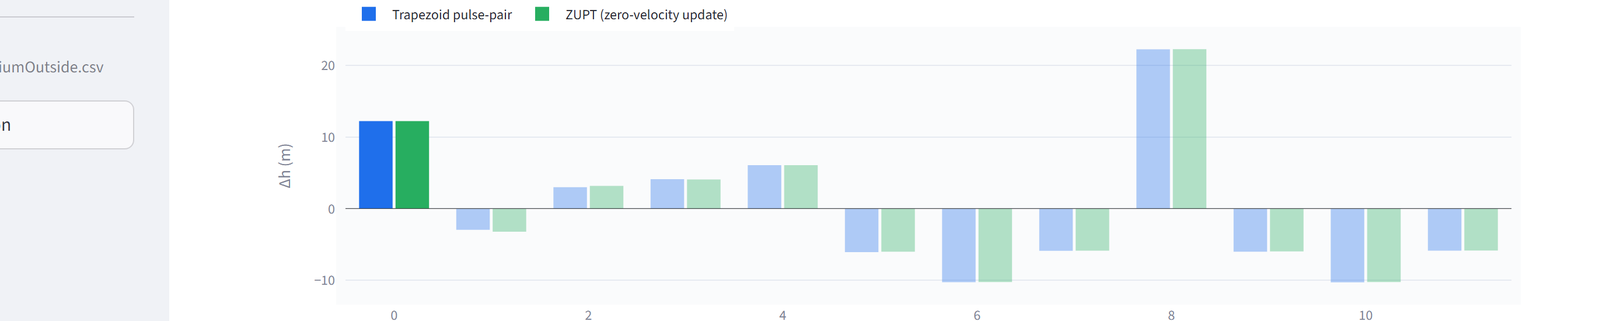
\includegraphics[width=\linewidth]{boutique/crops/clean_step4_metrics.png}
\end{minipage}\hfill
\begin{minipage}[t]{0.49\linewidth}
\centering
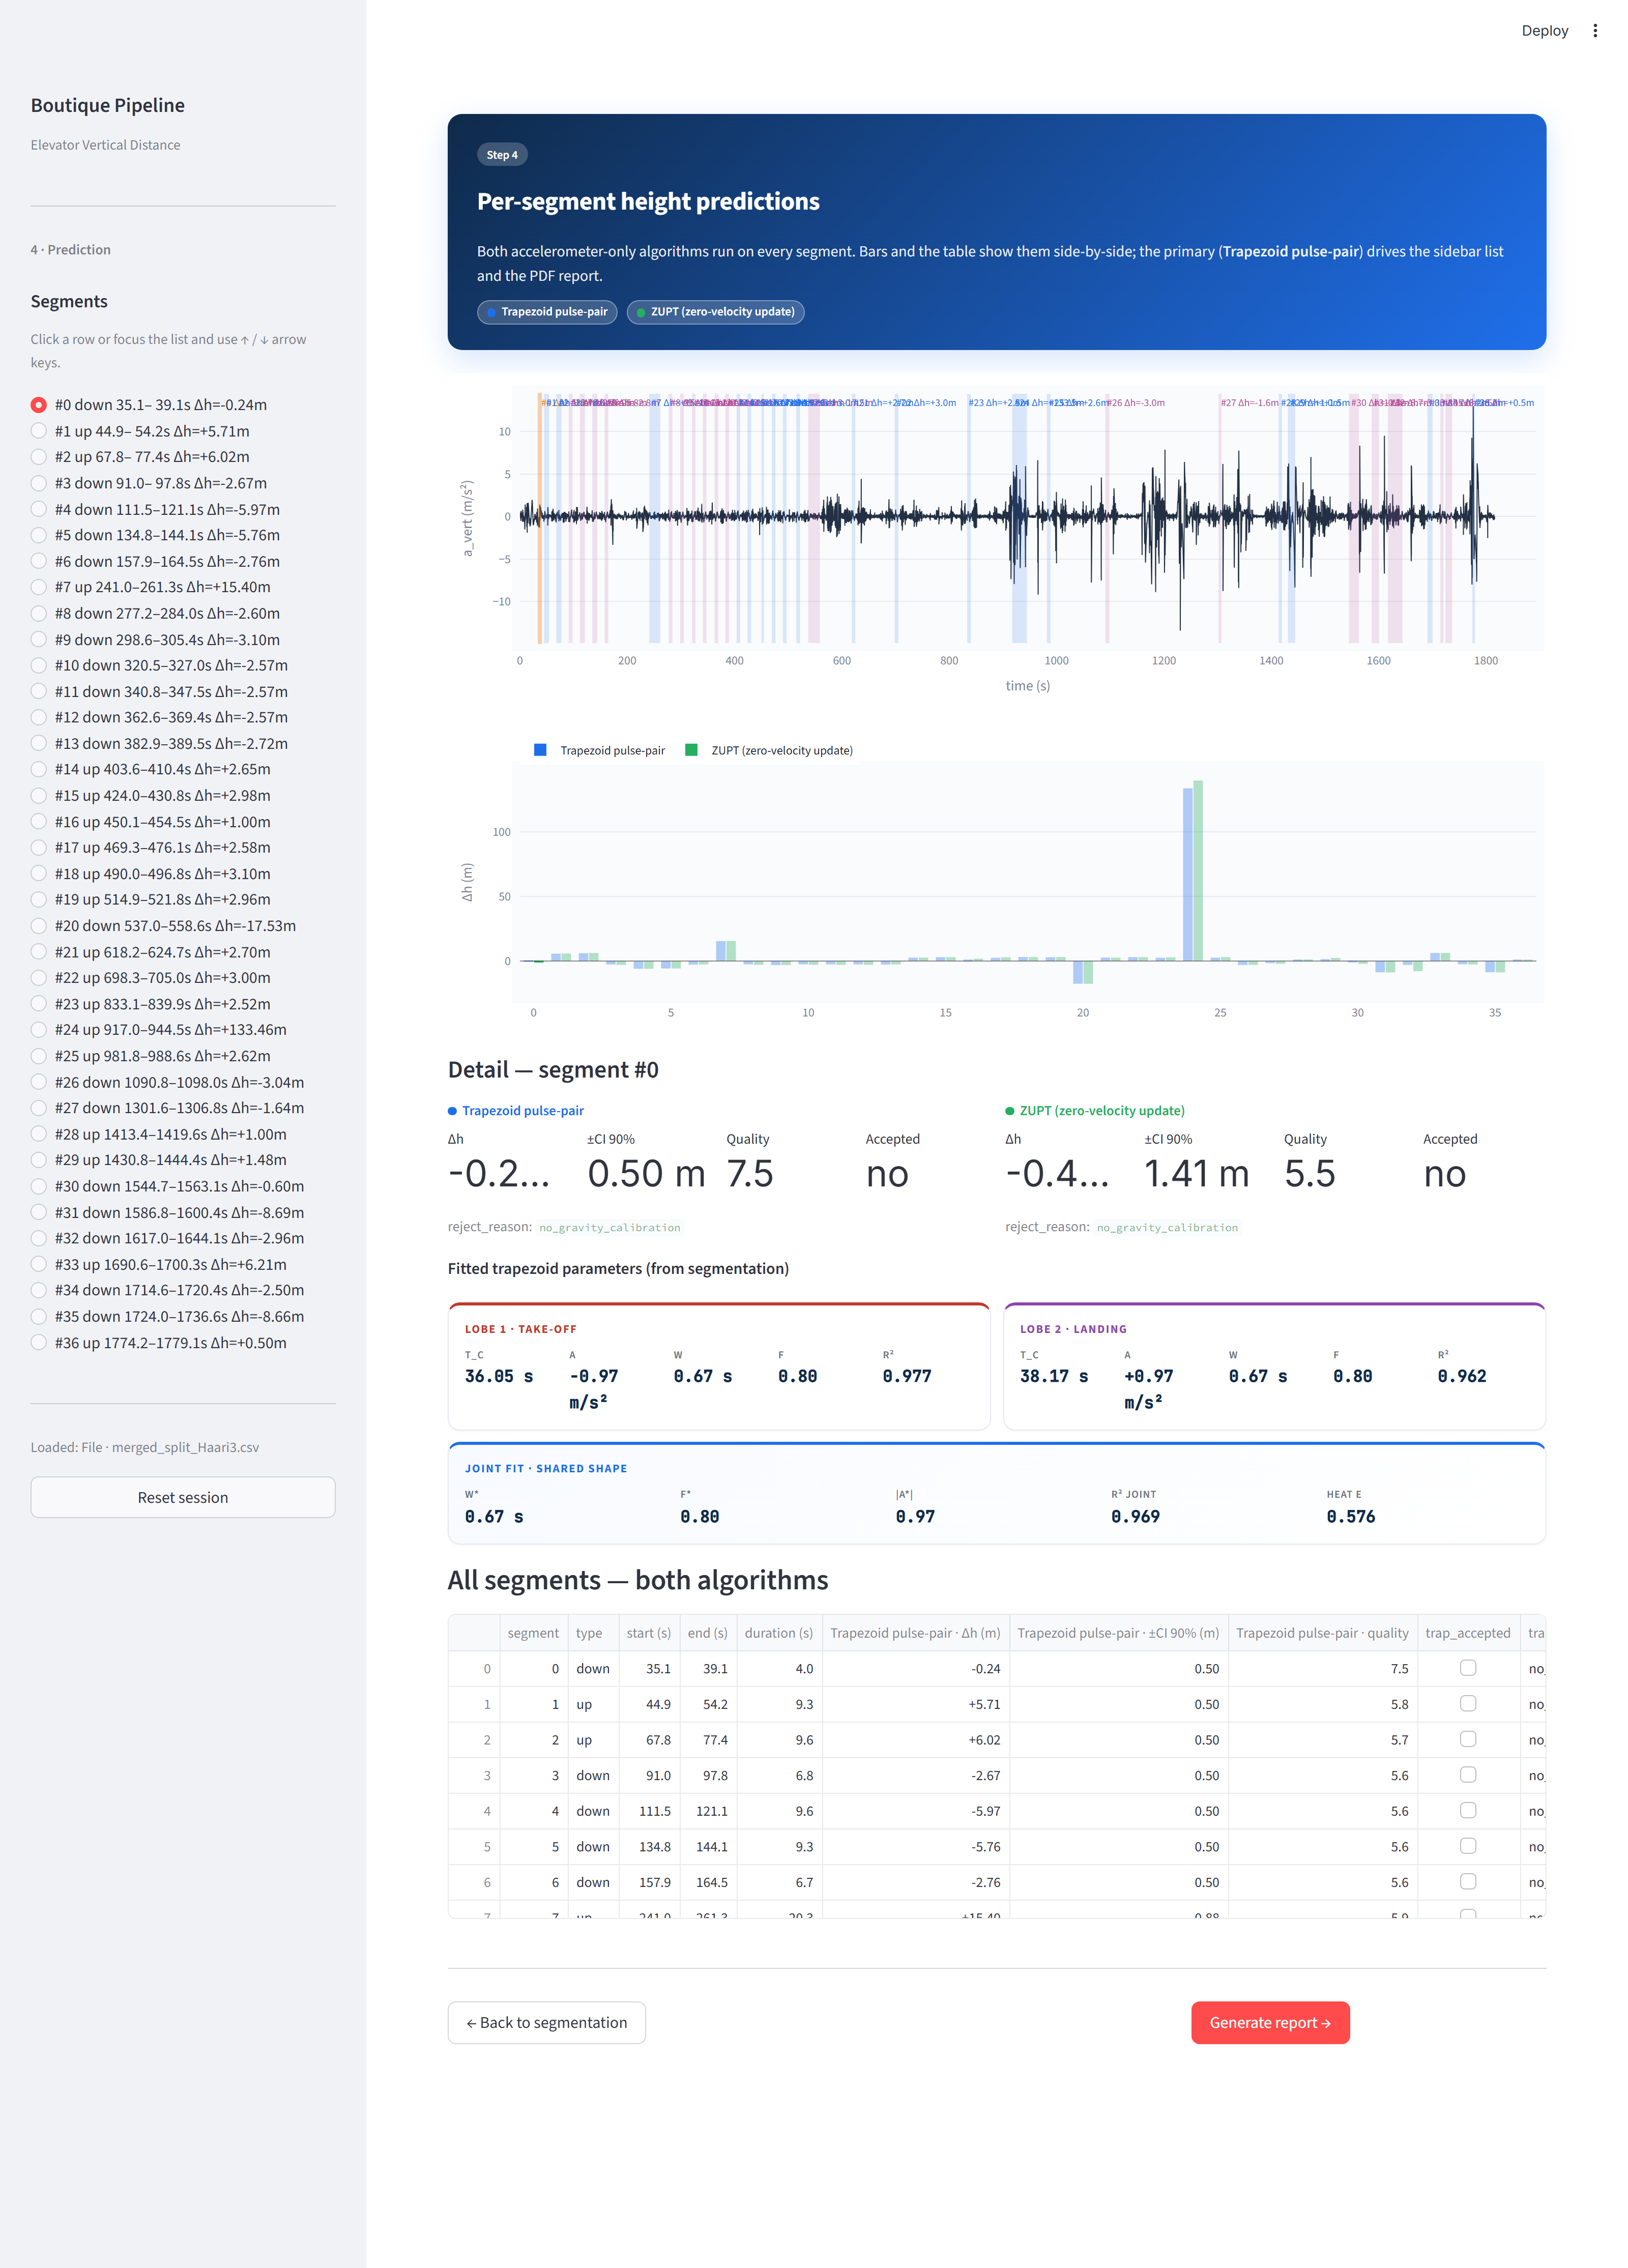
\includegraphics[width=\linewidth]{boutique/haari_step4_overview.png}
\end{minipage}
\caption{\textbf{תרשים העמודות בשלב 4.} \textenglish{Trapezoid}
(כחול) ו-\textenglish{ZUPT} (ירוק) זה לצד זה. \emph{שמאל
(\textcolor{green!50!black}{טוב}):} העמודות לכל מקטע כמעט זהות
בגובה לשני האלגוריתמים. הנסיעה הגדולה (\#8, $\Delta h \approx
+22$\,\textenglish{m}) תואמת. רמת ביטחון גבוהה בדו"ח.
\emph{ימין (\textcolor{red!70!black}{לחקור}):} כמה מקטעים מציגים
פערים גדולים בין הכחול לירוק. כל פער $>1.5$\,\textenglish{m}
הוא רמז לרעש או לגבולות שגויים (\autoref{sec:heb-fixing}); חוזרים
לשלב 3, מתקנים את המקטע, מנבאים שוב.}
\label{fig:hb-step4-cleanvshaari}
\end{figure}

\paragraph{פרטי המקטע הנבחר.}
לחיצה על מקטע מציגה ארבעה מספרים לכל אלגוריתם:

\begin{itemize}
  \item $\Delta h$ --- גובה עם סימן (\textenglish{m}).
  \item \textenglish{$\pm$CI 90\%} --- חצי-רוחב של רווח סמך 90\%.
    קטן יותר טוב יותר; היעד התכנוני קטן מ-1.5\,\textenglish{m}
    בנסיעות קצרות.
  \item \textenglish{Quality} --- ציון איכות; גבוה יותר טוב יותר.
  \item \textenglish{Accepted} --- כן/לא. ``לא'' מלווה ב-
    \textenglish{\texttt{reject\_reason}}.
\end{itemize}

מקטע שנדחה (\textenglish{Accepted: no}) עדיין מופיע בדו"ח אך
מסומן. \textenglish{\texttt{r2\_below\_thr}} פירושו ש-$R^2$ של
התאמת הטרפז המשותפת היה נמוך מדי;
\textenglish{\texttt{score\_above\_quantile}} פירושו שציון
ה-$\sigma$ למקטע נפל בקצה הימני של התפלגות הקליברציה. בשני
המקרים המספר מדווח אך יש להתייחס אליו כבעל ביטחון נמוך.

% =====================================================================
\section{מה מקבלים בסוף: דו"ח ה-PDF העברי}
\label{sec:heb-report}

שלב 5 מפיק קובץ \textenglish{PDF} בעברית בפורמט \textenglish{A4}.
עמוד שער (מטא-נתוני המקור, סיכום, גרף סקירה, וטבלת מקטעים), ועמוד
אחד לכל נסיעה (כותרת עם $\Delta h$ / רווח סמך / איכות / התקבל,
שכבת טרפז, וגרף מתאם בחלון $\pm 30$\,\textenglish{s}). העמוד
האחרון הוא מסביר עברי של המדדים, כדי שהנמען יוכל לקרוא בלי לקרוא
את המדריך הזה. שם הקובץ:
\textenglish{\texttt{boutique\_report\_YYYYMMDDTHHMMSSZ.pdf}}.

% =====================================================================
\section{מתקדם --- רק אם צריך לחפור}
\label{sec:heb-advanced}

הסעיף הזה אוסף כלי אבחון, קריאת פרמטרים ועצות למקרי קצה שהמשתמש
הרגיל יכול לדלג עליהם בבטחה. הוא כאן בשביל המפעיל שרוצה לוודא
מקטע גבולי לפני החלטה לשמור או למחוק.

\subsection{כרטיס פרמטרי הטרפז}
\label{sec:heb-paramcard}

מתחת לחלונית הטרפז, שלושה כרטיסים זה לצד זה מסכמים את ההתאמה
מבחינה מספרית.

\begin{figure}[H]
\centering

\includegraphics[width=0.95\linewidth]{boutique/panels/clean_step3_overview__params.png}
\caption{\textbf{כרטיס פרמטרים.} שדות לאונה 1 (המראה) ולאונה 2
(נחיתה): $t_c$ זמן מרכז, $A$ שיא מסומן, $W$ חצי-רוחב, $f$ שבר
\textenglish{plateau}, $R^2$ איכות מקומית. בשורת ההתאמה
המשותפת: $W^\star, f^\star$ של הצורה המשותפת ו-$R^2$ ואנרגית
מפת החום. בדיקות שפיות: לאונה 1 $A > 0$ בנסיעת \textenglish{up}
(הפוך ל-\textenglish{down}); $|A_1|$ ו-$|A_2|$ בתוך פער של
$\sim 30\%$; $R^2$ משותף מעל $\sim 0.85$ הוא הטווח שבו החיזוי
תוקף.}
\label{fig:hb-param-card}
\end{figure}

\subsection{הטבלה הרחבה להשוואת אלגוריתמים}

מתחת לתרשים העמודות, הטבלה מציגה כל מקטע עם
$\Delta h$ / רווח סמך / איכות / קבלה לשני האלגוריתמים זה לצד זה.
המדד השימושי ביותר הוא ההפרש לפי שורה:
$\Delta h_{\mathrm{trap}} - \Delta h_{\mathrm{ZUPT}}$.
פער של $> 1.5$\,\textenglish{m} הוא כמעט תמיד מקטע רועש או גבולות
שגויים --- אותם דפוסים שכבר אובחנו בשלב 3.

\subsection{מתי להשתמש ב-Trapezoid ומתי ב-ZUPT}

\begin{itemize}
  \item \textbf{\textenglish{Trapezoid pulse-pair}} (המספר הכותרתי
    בדו"ח). מתאים פרופיל \textenglish{S-curve} בעל שבעה קטעי
    מהירות לעקבת התאוצה הדו-אונתית. אמין על נסיעות נקיות; מומלץ
    לדו"ח.
  \item \textbf{\textenglish{ZUPT}.} אינטגרציה כפולה של התאוצה
    אחרי קיבוע מהירויות אפס בקצוות. אמין בנסיעות \emph{קצרות
    מאוד} שבהן למודל הטרפז אין מספיק דגימות; פחות אמין בנסיעות
    ארוכות שבהן זחילת אינטגרציה דומיננטית.
\end{itemize}

ה-\textenglish{PDF} משתמש בתוצאת \textenglish{Trapezoid} כמספר
הכותרתי. ה-\textenglish{ZUPT} מוצג בשלב 4 בלבד כבדיקת שפיות.

\subsection{הקלטות רועשות: שלושה משטרי כשל}

\paragraph{מוחלש (טלפון בכיס/תיק).}
תסמין: גרף המתאם המסומן ברובו אפור; משרעת הטרפז
$<0.5\,\mathrm{m/s}^2$ (\autoref{fig:hb-trap-bad-damped});
ארגמקס במפת חום בקצה. מוסיפים מקטעים שפוספסו ידנית אם יש לכם
אמת חיצונית (חיישן לחץ, וידיאו, סטופר); מודל ה-$\sigma$ של
החיזוי ירחיב את רווח הסמך אוטומטית.

\paragraph{טלפון רועד-יד / שיחה.}
תסמין: הרבה נקודות כתומות (\textenglish{unpaired}) וסגולות
(\textenglish{NMS}) משולבות בירוקות; תרשים העמודות מציג
``נסיעה'' או שתיים חשודות-קצרות ($<$1\,\textenglish{m}) סביב
הנסיעות האמיתיות. מוחקים את המקטעים החשודים.

\paragraph{מיזוג אויר / חבטת דלת.}
תסמין: עקבת התאוצה תחת אירוע מיזוג אויר טהור היא שטוחה, אך
חתך \textenglish{outside} מבוסס לחץ עלול ליפול ליד נחיתות
מעלית. בודקים נקודתית את גבולות המקטעים.

\subsection{עריכה מרובה ואיפוס}

ה-\textenglish{Spreadsheet editor (advanced)} בתחתית עמוד
הסגמנטציה מאפשר עריכה כטבלה, נוח לעריכות מרובות. הכפתור
\textenglish{Reset to detector output} מאפס את כל העריכות
הידניות ומריץ מחדש את הגלאי הדטרמיניסטי --- רשת ביטחון לעריכה
שהשתבשה.

\subsection{רשימת בדיקה לפני שליחת דו"ח}

שש בדיקות-עין שלוקחות פחות מדקה ומספיקות כדי לאשר דו"ח לשליחה:

\begin{enumerate}
  \item כל רצועה בגרף העליון מכסה צורת שתי-אונות נראית-לעין, ואין
    אונות שפוספסו בין רצועות.
  \item גרף המתאם של כל מקטע שנבחר מציג שתי נקודות ירוקות.
  \item ארגמקס מפת החום של כל מקטע נבחר נמצא בתוך הגריד (לא
    צמוד לקצה).
  \item שכבת הטרפז של כל מקטע נבחר יושבת על המעטפת המוחלקת.
  \item שני האלגוריתמים מסכימים על $\Delta h$ עד כדי
    $\sim 1$\,\textenglish{m}, וה-\textenglish{Trapezoid} מסמן
    \textenglish{accepted}.
  \item רווח סמך מתחת ל-$\sim 1.5$\,\textenglish{m} בנסיעות עד
    $\sim 10$\,\textenglish{s} ומתחת ל-$\sim 3$\,\textenglish{m}
    בארוכות ביותר.
\end{enumerate}

כששש הבדיקות עוברות, ה-\textenglish{PDF} מוכן לשליחה. כששתיים
או יותר נכשלות על מקטע יחיד, זה המקטע לטפל בו ראשון; שאר הדו"ח
לרוב לא מושפע.

\subsection{שאלות נפוצות}

\paragraph{הגלאי לא החזיר אף סגמנט.}
או שההקלטה לא מכילה נסיעות, או שהנסיעות קצרות מהסף, או שהאות
מוחלש מתחת לסף המשרעת. \textenglish{$+$ Add segment} מסרגל הצד
ועריכה ידנית.

\paragraph{יותר מדי סגמנטים.}
הקלטה רועדת/הליכה. ממיינים את תרשים העמודות בשלב 4 לפי איכות
ומוחקים את הנמוכים.

\paragraph{אלגוריתמים נחלקים בפער $>1.5$\,\textenglish{m} על מקטע.}
מחתכים מחדש את גבולות המקטע (\autoref{sec:heb-fixing}, דפוס ד׳)
ומנבאים שוב.

\paragraph{האיכות אומרת ``\textenglish{Accepted: no}''.}
קוראים את ה-\textenglish{\texttt{reject\_reason}}. שתי הסיבות
הנפוצות (\textenglish{\texttt{r2\_below\_thr}},
\textenglish{\texttt{score\_above\_quantile}}) הן אותות הוגנים
--- הערך מדווח אך יש להתייחס אליו כבעל ביטחון נמוך.

\paragraph{כפתור ההורדה אפור.}
לא סיימתם את שלב 4. חוזרים, לוחצים \textenglish{Generate report},
ומנסים שוב.

\paragraph{אפשר להריץ את הפייפליין מקוד?}
כן; מחלקות \textenglish{\texttt{Segmenter}} ו-
\textenglish{\texttt{Predictor}} מיובאות ישירות.
ה-\textenglish{Streamlit} הוא רק שכבת תצוגה דקה.

\end{document}
